% Options for packages loaded elsewhere
\PassOptionsToPackage{unicode}{hyperref}
\PassOptionsToPackage{hyphens}{url}
\PassOptionsToPackage{dvipsnames,svgnames,x11names}{xcolor}
%

\documentclass{juliacon}

\usepackage{amsmath,amssymb}
\usepackage{setspace}
\usepackage{iftex}
\ifPDFTeX
  \usepackage[T1]{fontenc}
  \usepackage[utf8]{inputenc}
  \usepackage{textcomp} % provide euro and other symbols
\else % if luatex or xetex
  \usepackage{unicode-math}
  \defaultfontfeatures{Scale=MatchLowercase}
  \defaultfontfeatures[\rmfamily]{Ligatures=TeX,Scale=1}
\fi
\usepackage[]{tgtermes}
\ifPDFTeX\else  
    % xetex/luatex font selection
\fi
% Use upquote if available, for straight quotes in verbatim environments
\IfFileExists{upquote.sty}{\usepackage{upquote}}{}
\IfFileExists{microtype.sty}{% use microtype if available
  \usepackage[]{microtype}
  \UseMicrotypeSet[protrusion]{basicmath} % disable protrusion for tt fonts
}{}
\makeatletter
\@ifundefined{KOMAClassName}{% if non-KOMA class
  \IfFileExists{parskip.sty}{%
    \usepackage{parskip}
  }{% else
    \setlength{\parindent}{0pt}
    \setlength{\parskip}{6pt plus 2pt minus 1pt}}
}{% if KOMA class
  \KOMAoptions{parskip=half}}
\makeatother
\usepackage{xcolor}
\setlength{\emergencystretch}{3em} % prevent overfull lines
\setcounter{secnumdepth}{5}
% Make \paragraph and \subparagraph free-standing
\ifx\paragraph\undefined\else
  \let\oldparagraph\paragraph
  \renewcommand{\paragraph}[1]{\oldparagraph{#1}\mbox{}}
\fi
\ifx\subparagraph\undefined\else
  \let\oldsubparagraph\subparagraph
  \renewcommand{\subparagraph}[1]{\oldsubparagraph{#1}\mbox{}}
\fi


\providecommand{\tightlist}{%
  \setlength{\itemsep}{0pt}\setlength{\parskip}{0pt}}\usepackage{longtable,booktabs,array}
\usepackage{calc} % for calculating minipage widths
% Correct order of tables after \paragraph or \subparagraph
\usepackage{etoolbox}
\makeatletter
\patchcmd\longtable{\par}{\if@noskipsec\mbox{}\fi\par}{}{}
\makeatother
% Allow footnotes in longtable head/foot
\IfFileExists{footnotehyper.sty}{\usepackage{footnotehyper}}{\usepackage{footnote}}
\makesavenoteenv{longtable}
\usepackage{graphicx}
\makeatletter
\def\maxwidth{\ifdim\Gin@nat@width>\linewidth\linewidth\else\Gin@nat@width\fi}
\def\maxheight{\ifdim\Gin@nat@height>\textheight\textheight\else\Gin@nat@height\fi}
\makeatother
% Scale images if necessary, so that they will not overflow the page
% margins by default, and it is still possible to overwrite the defaults
% using explicit options in \includegraphics[width, height, ...]{}
\setkeys{Gin}{width=\maxwidth,height=\maxheight,keepaspectratio}
% Set default figure placement to htbp
\makeatletter
\def\fps@figure{htbp}
\makeatother

% Keywords command
\providecommand{\JCONkeywords}[1]
{
  \small	
  \section*{Keywords} #1
}

% Two-column table
% Lifted from https://github.com/quarto-journals/elsevier/blob/main/_extensions/elsevier/partials/_two-column-longtable.tex.
\usepackage{float}
\makeatletter
\let\oldlt\longtable
\let\endoldlt\endlongtable
\def\longtable{\@ifnextchar[\longtable@i \longtable@ii}
\def\longtable@i[#1]{\begin{figure}[H]
\onecolumn
\begin{minipage}{0.5\textwidth}
\oldlt[#1]
}
\def\longtable@ii{\begin{figure}[H]
\onecolumn
\begin{minipage}{0.5\textwidth}
\oldlt
}
\def\endlongtable{\endoldlt
\end{minipage}
\twocolumn
\end{figure}}
\makeatother

% Remove whitespace after paragraphs
\setlength{\parskip}{0pt}

\bibliographystyle{juliacon}
\usepackage{orcidlink}
\definecolor{mypink}{RGB}{219, 48, 122}
\makeatletter
\makeatother
\makeatletter
\makeatother
\makeatletter
\@ifpackageloaded{caption}{}{\usepackage{caption}}
\AtBeginDocument{%
\ifdefined\contentsname
  \renewcommand*\contentsname{Table of contents}
\else
  \newcommand\contentsname{Table of contents}
\fi
\ifdefined\listfigurename
  \renewcommand*\listfigurename{List of Figures}
\else
  \newcommand\listfigurename{List of Figures}
\fi
\ifdefined\listtablename
  \renewcommand*\listtablename{List of Tables}
\else
  \newcommand\listtablename{List of Tables}
\fi
\ifdefined\figurename
  \renewcommand*\figurename{Figure}
\else
  \newcommand\figurename{Figure}
\fi
\ifdefined\tablename
  \renewcommand*\tablename{Table}
\else
  \newcommand\tablename{Table}
\fi
}
\@ifpackageloaded{float}{}{\usepackage{float}}
\floatstyle{ruled}
\@ifundefined{c@chapter}{\newfloat{codelisting}{h}{lop}}{\newfloat{codelisting}{h}{lop}[chapter]}
\floatname{codelisting}{Listing}
\newcommand*\listoflistings{\listof{codelisting}{List of Listings}}
\makeatother
\makeatletter
\@ifpackageloaded{caption}{}{\usepackage{caption}}
\@ifpackageloaded{subcaption}{}{\usepackage{subcaption}}
\makeatother
\makeatletter
\@ifpackageloaded{tcolorbox}{}{\usepackage[skins,breakable]{tcolorbox}}
\makeatother
\makeatletter
\@ifundefined{shadecolor}{\definecolor{shadecolor}{rgb}{.97, .97, .97}}
\makeatother
\makeatletter
\makeatother
\makeatletter
\makeatother
\ifLuaTeX
  \usepackage{selnolig}  % disable illegal ligatures
\fi
\usepackage[]{biblatex}
\addbibresource{ref.bib}
\IfFileExists{bookmark.sty}{\usepackage{bookmark}}{\usepackage{hyperref}}
\IfFileExists{xurl.sty}{\usepackage{xurl}}{} % add URL line breaks if available
\urlstyle{same} % disable monospaced font for URLs
\hypersetup{
  pdftitle={Effortless Bayesian Deep Learning in Julia through Laplace},
  pdfkeywords={Julia, Probabilistic Machine Learning, Laplace
Approximation, Deep Learning, Artificial Intelligence},
  colorlinks=true,
  linkcolor={blue},
  filecolor={Maroon},
  citecolor={Blue},
  urlcolor={Blue},
  pdfcreator={LaTeX via pandoc}}


\title{Effortless Bayesian Deep Learning in Julia through Laplace}

\author[1]{Patrick Altmeyer}
\affil[1]{Delft University of Technology}
\date{2023-11-17}
\begin{document}
\maketitle

% Abstract
\begin{abstract}

Treating deep neural networks probabilistically comes with numerous
advantages including improved robustness and greater interpretability.
These factors are key to building Artificial Intelligence (AI) that is
trustworthy. A drawback commonly associated with existing Bayesian
methods is that they increase computational costs. Recent work has shown
that Bayesian deep learning can be effortless through Laplace
approximation. We propose a small Julia package,
\texttt{LaplaceRedux.jl} that implements this new approach for deep
neural networks trained in \texttt{Flux.jl}.
\end{abstract}

% Keywords
\JCONkeywords{Julia, Probabilistic Machine Learning, Laplace
Approximation, Deep Learning, Artificial Intelligence}

% Hypersetup
\hypersetup{
    pdftitle = {Effortless Bayesian Deep Learning in Julia through
Laplace},
    pdfsubject = {JuliaCon \@year Proceedings},
    pdfauthor = {},
    pdfkeywords = {Julia, Probabilistic Machine Learning, Laplace
Approximation, Deep Learning, Artificial Intelligence},
}

\setcounter{page}{1}

\ifdefined\Shaded\renewenvironment{Shaded}{\begin{tcolorbox}[interior hidden, breakable, sharp corners, enhanced, boxrule=0pt, frame hidden, borderline west={3pt}{0pt}{shadecolor}]}{\end{tcolorbox}}\fi

\setstretch{1}
\hypertarget{sec-intro}{%
\section{Background}\label{sec-intro}}

Over the past decade, Deep Learning (DL) has arguably been one of the
dominating subdisciplines of Artificial Intelligence. Despite the
tremendous success of deep neural networks, practitioners and
researchers have also pointed to a vast number of pitfalls that have so
far inhibited the use of DL in safety-critical applications. Among other
things, these pitfalls include a lack of adversarial robustness
\autocite{goodfellow2014explaining} and an inherent opaqueness of deep
neural networks, often described as the black-box problem.

In deep learning, the number of parameters relative to the size of the
available data is generally huge:

\begin{quote}
{[}\ldots{]} deep neural networks are typically very underspecified by
the available data, and {[}\ldots{]} parameters {[}therefore{]}
correspond to a diverse variety of compelling explanations for the data.
\textcite{wilson2020case}
\end{quote}

A scenario like this very much calls for treating model predictions
probabilistically \autocite{wilson2020case}. It is therefore not
surprising that interest in Bayesian deep learning has grown in recent
years as researchers have tackled the problem from a wide range of
angles including MCMC (see
\href{https://turing.ml/dev/tutorials/03-bayesian-neural-network/}{\texttt{Turing}}),
Mean Field Variational Inference \autocite{blundell2015weight}, Monte
Carlo Dropout \autocite{gal2016dropout} and Deep Ensembles
\autocite{lakshminarayanan2016simple}. Laplace Redux
\autocite{immer2020improving,daxberger2021laplace} is one of the most
recent and promising approaches to Bayesian neural networks (BNN).

\hypertarget{sec-body}{%
\section{Laplace Approximation for Deep Learning}\label{sec-body}}

Let \(\mathcal{D}=\{x,y\}_{n=1}^N\) denote our feature-label pairs and
let \(f(x;\theta)=y\) denote some deep neural network specified by its
parameters \(\theta\). We are interested in estimating the posterior
predictive distribution given by the following Bayesian model average
(BMA):

\begin{equation}\protect\hypertarget{eq-bma}{}{
p(y|x,\mathcal{D}) = \int p(y|x,\theta)p(\theta|\mathcal{D})d\theta
}\label{eq-bma}\end{equation}

To do so we first need to compute the weight posterior
\(p(\theta|\mathcal{D})\). Laplace Approximation (LA) relies on the fact
that the second-order Taylor expansion of this posterior amounts to a
multivariate Gaussian \(q(\theta)=\mathcal{N}(\hat\mu,\hat\Sigma)\)
centred around the maximum a posteriori (MAP) estimate
\(\hat\mu=\hat{\theta}=\arg\max_{\theta}p(\theta|\mathcal{D})\) with
covariance equal to the negative inverse Hessian of our loss function
evaluated at the mode
\(\hat{\Sigma}=-(\hat{\mathcal{H}}|_{\hat{\theta}})^{-1}\).

To apply Laplace in the context of deep learning, we can train our
network in the standard way by minimizing the negative log-likelihood
\(\ell(\theta)=-\log p(y|x,\mathcal{D})\). To obtain Gaussian LA weight
posterior we then only need to compute the Hessian evaluated at the
obtained MAP estimate.

Laplace Approximation itself dates back to the 18th century, but despite
its simplicity, it has not been widely used or studied by the deep
learning community until recently. One reason for this may be that for
large neural networks with many parameters, the exact Hessian
computation is prohibitive. One can rely on linearized approximations of
the Hessian, but those still scale quadratically in the number of
parameters. Fortunately, recent work has shown that block-diagonal
factorizations can be successfully applied in this context
\autocite{martens2015optimizing}.

Another reason why LA may have been neglected in the past is that early
attempts at using it for deep learning failed: simply sampling from the
Laplace posterior to compute the exact BNN posterior predictive
distribution in Equation~\ref{eq-bma} does not work when using
approximations for the Hessian \autocite{lawrence2001variational}.
Instead, we can use a linear expansion of the predictive around the mode
as demonstrated by \textcite{immer2020improving}. Formally, we locally
linearize our network,

\begin{equation}\protect\hypertarget{eq-glm}{}{
f^{\hat{\theta}}_{\mbox{lin}}(x;\theta)=f(x;\hat{\theta}) + \mathcal{J}_{\theta}(\theta-\hat{\theta})
}\label{eq-glm}\end{equation}

which turns the BNN into a Bayesian generalized linear model (GLM) where
\(\hat{\theta}\) corresponds to the MAP estimate as before. The
corresponding GLM predictive,

\begin{equation}\protect\hypertarget{eq-glm-predictive}{}{
p(y|x,\mathcal{D}) = \mathbb{E} \left[ p(y|f^{\hat{\theta}}_{\mbox{lin}}(x;\theta_n)) \right], \ \ \ \theta_n \sim q(\theta)
}\label{eq-glm-predictive}\end{equation}

has a closed-form solution for regression problems. For classification
problems it can be approximated using (extended) probit approximation
\autocite{daxberger2021laplace}.

\textcite{immer2020improving} provide a much more detailed exposition of
the above with a focus on theoretical underpinnings and intuition.
\textcite{daxberger2021laplace} introduce Laplace Redux from more of an
applied perspective and present a comprehensive Python implementation:
\href{https://aleximmer.github.io/Laplace/}{laplace}.

\hypertarget{laplaceredux.jl-a-julia-implementation}{%
\section{\texorpdfstring{\texttt{LaplaceRedux.jl} --- a Julia
implementation}{LaplaceRedux.jl --- a Julia implementation}}\label{laplaceredux.jl-a-julia-implementation}}

The \texttt{LaplaceRedux.jl} package is intended to make this new
methodological framework available to the Julia community. It is
interfaced with the popular deep learning library,
\href{https://fluxml.ai/}{\texttt{Flux.jl}}.

Using just a few lines of code the package enables users to compute and
apply Laplace Redux to their pre-trained neural networks. A basic usage
example is shown in listing \ref{lst:laplace}: the \texttt{Laplace}
function simply wraps the Flux neural network \texttt{nn}. The returned
instance is then fitted to data using the generic \texttt{fit!} method.
Finally, the prior precision \(\lambda\) is optimized through Empirical
Bayes \autocite{daxberger2021laplace}. Calling the generic
\texttt{predict} method on the fitted instance will generate GLM
predictions according to Equation~\ref{eq-glm-predictive}.

\begin{lstlisting}[language=Julia, escapechar=@, numbers=left, label={lst:laplace}, caption={}]
la = Laplace(nn; likelihood=:classification)
fit!(la, data)
optimize_prior!(la)
\end{lstlisting}

Figure~\ref{fig-class} shows an example involving a synthetic data set
consisting of two classes. Contours indicate the predicted probabilities
using the plugin estimator (left), untuned Laplace Approximation
(center) and finally optimized LA (right). For the latter two, the
respective choices for the prior precision parameter \(\lambda\) are
indicated in the title. Relying solely on the MAP estimate, the plugin
estimator produces overly confident predictions. Conversely, the GLM
predictions account for predictive uncertainty as captured by the
Laplace posterior.

Figure~\ref{fig-reg} presents a regression example with optimized LA.
Wide regions of the confidence interval (shaded area) indicate high
predictive uncertainty. Intuitively, the estimated predictive
uncertainty increases significantly in regions characterized by high
epistemic uncertainty: epistemic uncertainty arises in regions of the
domain that have not been observed by the classifier, so regions that
are free of training samples.

\begin{figure}

{\centering 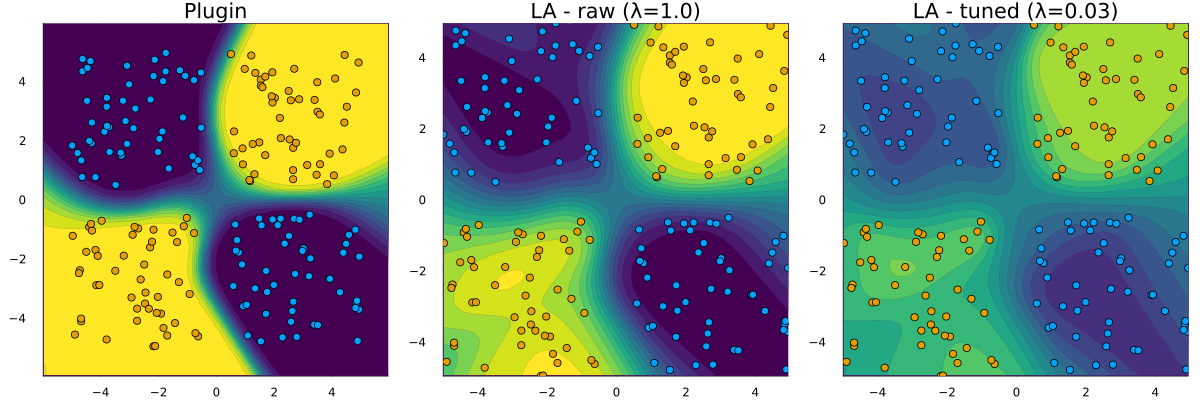
\includegraphics[width=3.33333in,height=1.11667in]{www/posterior_predictive_mlp.png}

}

\caption{\label{fig-class}Posterior predictive distribution for binary
classifier: plugin estimate (left), untuned LA (center) and optimized LA
(right). The colour of the contour indicates the predicted class
probabilities: the more yellow a region, the more confident the
classifier that samples belong to the orange class.}

\end{figure}

\begin{figure}

{\centering 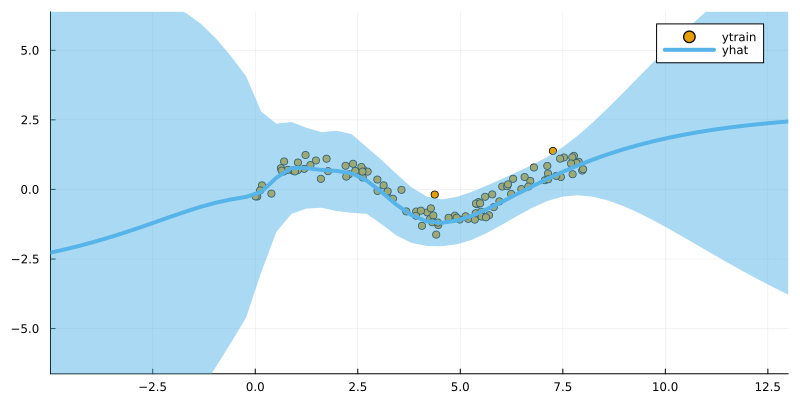
\includegraphics[width=3.33333in,height=1.66667in]{www/regression.png}

}

\caption{\label{fig-reg}Posterior predictive distribution for regressor:
wide regions of the confidence interval (shaded area) indicate high
predictive uncertainty.}

\end{figure}

\hypertarget{sec-con}{%
\section{Discussion and Outlook}\label{sec-con}}

At the time of writing, the package is still in its infancy and its
functionality is limited. It currently lacks multi-class support and
still works with full Hessian approximations, as opposed to the less
expensive (block-) diagonal variants. That being said, choices regarding
the package architecture were made with these future development
opportunities in mind. This should hopefully make the package attractive
to other Julia developers interested in the topic.

Laplace Redux is an exciting and promising recent development in
Bayesian deep learning. The goal of this project is to bring this
framework to the attention of the Julia machine-learning community. The
package \texttt{LaplaceRedux.jl} offers a starting ground for a
full-fledged implementation in pure Julia. Future developments are
planned and contributions are very much welcome.

\hypertarget{sec-ack}{%
\section{Acknowledgements}\label{sec-ack}}

I am grateful to my PhD supervisors Cynthia C. S. Liem and Arie van
Deursen for being so supportive of my work on open-source developments.
I am also grateful to the Julia community for being so kind, welcoming
and helpful.


\printbibliography


\end{document}
